\documentclass{mwhittaker}
\title{Bipartisan Paxos}

\usepackage{algorithmicx}
\usepackage{algorithm}
\usepackage{algpseudocode}
\usepackage{appendix}
\usepackage{mdframed}
\usepackage{mdframed}
\usepackage{multirow}
\usepackage{pervasives}
\usepackage{subcaption}
\usepackage{tikz}
\usetikzlibrary{calc}
\usetikzlibrary{positioning}
\usetikzlibrary{shapes.misc}

% Boxed invariants.
\newmdtheoremenv[
  hidealllines=true,
  innerleftmargin=8pt,%
  innerrightmargin=8pt,%
  innertopmargin=0pt,%
  innerbottommargin=8pt,%
  backgroundcolor=flatblue!20,%
  skipbelow=\baselineskip,%
  skipabove=8pt]{boxedinvariant}{Invariant}

% Misc commands.
\newcommand{\deps}[1]{\text{deps}(#1)}
\newcommand{\noop}{\text{noop}}
\newcommand{\quorum}{\mathcal{Q}}
\newcommand{\superquorum}{\mathcal{S}}
\newcommand{\QuorumMajoritySize}{\floor{\frac{f}{2}} + 1}
\newcommand{\Pnoop}[1]{P^{\noop}_{#1}}
\newcommand{\Pnotnoop}[1]{P^{\lnot \noop}_{#1}}
\newcommand{\pruned}{\text{pruned}}

% Remove the "end if" from algorithmicx. See [1].
%
% [1]: https://tex.stackexchange.com/a/53518
\algtext*{EndIf}
\algtext*{EndFor}

% Misc styling.
\tikzstyle{square}=[%
  draw,
  line width=1pt,
  minimum height=0.5in,
  minimum width=0.5in,
  text width=0.4in,
  align=center
]

\begin{document}
\maketitle

% {\begin{abstract}
  In this paper, we present a family of state machine replication protocols
  inspired by Fast Paxos~\cite{lamport2006fast}, EPaxos~\cite{moraru2013there},
  and Caesar~\cite{arun2017speeding}. The protocols are called Bipartisan
  Paxos, Unanimous Bipartisan Paxos, and Majority Commit Bipartisan Paxos.
\end{abstract}

}
% {\section{Bipartisan Paxos}\seclabel{BipartisanPaxos}
In this section, we introduce \defword{Bipartisan Paxos}, or \defword{BPaxos}
for short. BPaxos is designed to be as simple to understand as possible, even
at the cost of performance. Other variants of BPaxos that we'll see later
(i.e.\ Unanimous BPaxos and Majority Commit BPaxos) improve on BPaxos'
performance.

\paragraph{Overview}
MultiPaxos allows a set of nodes to agree on a totally ordered sequence of
state machine commands. This is illustrated in \figref{MultiPaxosCartoon}.

\begin{figure}[h]
  \centering
  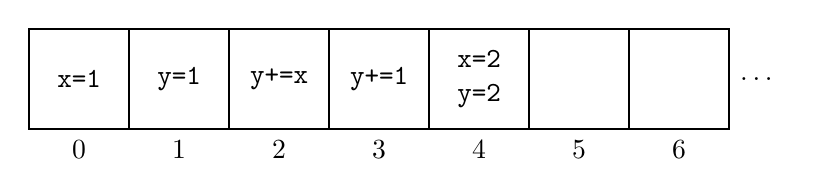
\begin{tikzpicture}
    \node[square] (a) at (0, 0) {\texttt{x=1}};
    \node[square, right=-1pt of a] (b) {\texttt{y=1}};
    \node[square, right=-1pt of b] (c) {\texttt{y+=x}};
    \node[square, right=-1pt of c] (d) {\texttt{y+=1}};
    \node[square, right=-1pt of d] (e) {\texttt{x=2\\y=2}};
    \node[square, right=-1pt of e] (f) {};
    \node[square, right=-1pt of f] (g) {};
    \node[right=0in of g] (h) {\ldots};

    \foreach \label/\i in {a/0, b/1, c/2, d/3, e/4, f/5, g/6} {%
      \node[below=0in of \label] {\i};
    }
  \end{tikzpicture}
  \caption{MultiPaxos}\figlabel{MultiPaxosCartoon}
\end{figure}

While simple, agreeing on a totally ordered sequence of state machine commands
can be overly prescriptive. If two commands conflict (e.g., \texttt{x = 1} and
\texttt{x = 2}), then they \emph{do} need to be executed by every state machine
replica in the same order. But, if two commands do \emph{not} conflict (e.g.,
\texttt{x = 1} and \texttt{y = 1}), then they do \emph{not} need to be totally
ordered.  State machine replicas can execute them in either order.

EPaxos takes advantage of this fact and attempts to order commands only if they
conflict. To do so, it ditches the totally ordered sequence and instead agrees
on a directed graph of commands such that every pair of conflicting commands
have an edge between them. An example is illustrated in \figref{EPaxosCartoon}%
\footnote{%
  In reality, the graph would be the transitive closure of the one in
  \figref{EPaxosCartoon}, but we do not draw all edges to keep things simple
}.
EPaxos then executes this graph in reverse topological order one strongly
connected component at a time, executing commands within a component in an
arbitrary but deterministic order. For example, in \figref{EPaxosCartoon}, we
could execute commands in the order $R.1, R.2, S.1, Q.2, Q.1$.

\begin{figure}[h]
  \centering
  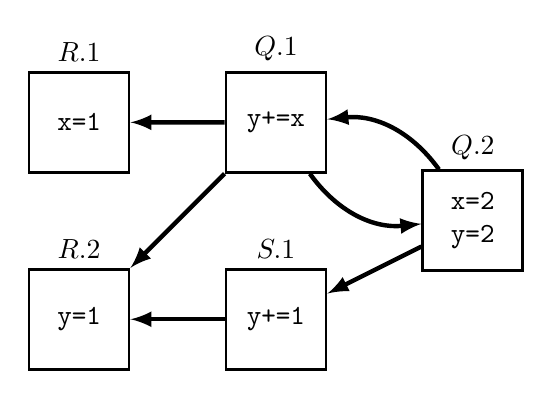
\begin{tikzpicture}[scale=2.5]
    \node[square] (a) at (0, 1) {\texttt{x=1}};
    \node[square] (b) at (0, 0) {\texttt{y=1}};
    \node[square] (c) at (1, 1) {\texttt{y+=x}};
    \node[square] (d) at (1, 0) {\texttt{y+=1}};
    \node[square] (e) at (2, 0.5) {\texttt{x=2\\y=2}};
    \draw[ultra thick, -latex] (c) to (a);
    \draw[ultra thick, -latex] (c) to (b);
    \draw[ultra thick, -latex, bend right] (c) to (e);
    \draw[ultra thick, -latex] (d) to (b);
    \draw[ultra thick, -latex, bend right] (e) to (c);
    \draw[ultra thick, -latex] (e) to (d);

    \foreach \label/\i in {a/$R.1$, b/$R.2$, c/$Q.1$, d/$S.1$, e/$Q.2$} {%
      \node[above=0in of \label] {\i};
    }
  \end{tikzpicture}
  \caption{EPaxos}\figlabel{EPaxosCartoon}
\end{figure}

Every vertex in the graph has a unique name like $Q.1$ or $R.1$. EPaxos calls
these \defword{instances}. We can view a named vertex, the command inside the
vertex, and the vertex's outbound edges as a little gadget. For example,
\figref{EPaxosGadgets} shows gadgets for instances $R.2$, $Q.1$, and $Q.2$.
%
More formally, we can think of these gadgets as tuples like $(Q.1,
\texttt{y+=x}, \set{R.1, R.2, Q.2})$ where $Q.1$ is the instance, \texttt{y+=x}
is the command in the instance, and the set $\set{R.1, R.2, Q.2}$ is the set of
\defword{dependencies} of $Q.1$ (or of \texttt{y+=x} if $Q.1$ is clear from
context).

\begin{figure}[h]
  \centering

  \begin{subfigure}[b]{0.19\textwidth}
    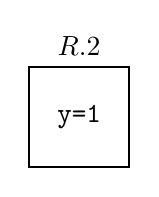
\begin{tikzpicture}[scale=2.5]
      \node[square] (b) at (0, 0) {\texttt{y=1}};
      \foreach \label/\i in {b/$R.2$} {%
        \node[above=0in of \label] {\i};
      }
    \end{tikzpicture}
  \end{subfigure}
  %
  \begin{subfigure}[b]{0.49\textwidth}
    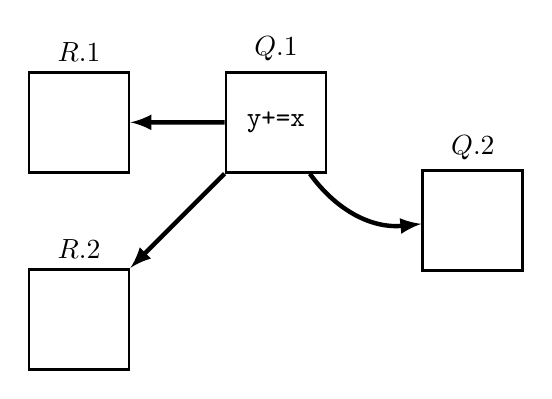
\begin{tikzpicture}[scale=2.5]
      \node[square] (a) at (0, 1) {};
      \node[square] (b) at (0, 0) {};
      \node[square] (c) at (1, 1) {\texttt{y+=x}};
      \node[square] (e) at (2, 0.5) {};
      \draw[ultra thick, -latex] (c) to (a);
      \draw[ultra thick, -latex] (c) to (b);
      \draw[ultra thick, -latex, bend right] (c) to (e);
      \foreach \label/\i in {a/$R.1$, b/$R.2$, c/$Q.1$, e/$Q.2$} {%
        \node[above=0in of \label] {\i};
      }
    \end{tikzpicture}
  \end{subfigure}
  %
  \begin{subfigure}[b]{0.29\textwidth}
    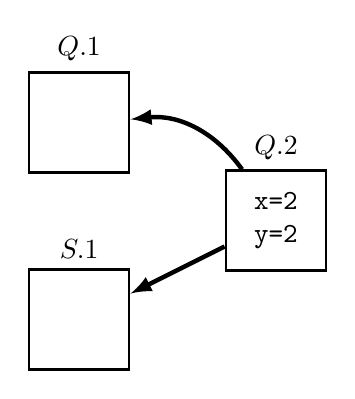
\begin{tikzpicture}[scale=2.5]
      \node[square] (c) at (1, 1) {};
      \node[square] (d) at (1, 0) {};
      \node[square] (e) at (2, 0.5) {\texttt{x=2\\y=2}};
      \draw[ultra thick, -latex, bend right] (e) to (c);
      \draw[ultra thick, -latex] (e) to (d);
      \foreach \label/\i in {c/$Q.1$, d/$S.1$, e/$Q.2$} {%
        \node[above=0in of \label] {\i};
      }
    \end{tikzpicture}
  \end{subfigure}

  \caption{EPaxos Gadgets}\figlabel{EPaxosGadgets}
\end{figure}

EPaxos nodes collectively construct the directed graph of commands by stitching
together a bunch of gadgets. More precisely, an EPaxos node $R$ proposes a
gadget for instance $R.i$ and attempts to get the gadget chosen. Once a gadget
is chosen, it is considered part of the directed graph and is eligible for
execution. EPaxos' correctness hinges on the following two key invariants
(later we'll see why these invariants ensure EPaxos' correctness).

\begin{boxedinvariant}\invlabel{GadgetsChosen}
  Once a gadget $(R.i, a, \deps{a})$ has been chosen, no other gadget can be
  chosen for instance $R.i$.
\end{boxedinvariant}

\begin{boxedinvariant}\invlabel{ConflictingGadgets}
  If two gadgets $(I_a, a, \deps{a})$ and $(I_b, b, \deps{b})$ are chosen and
  commands $a$ and $b$ conflict, then either $I_a \in \deps{b}$ or $I_b \in
  \deps{a}$ or both.
\end{boxedinvariant}

BPaxos, like EPaxos, also constructs a directed graph of commands and executes
them in reverse topological order one strongly connected component at a time.
In fact, BPaxos and EPaxos execute commands in 100\% the same way. BPaxos also
maintains the same two key invariants as EPaxos. BPaxos and EPaxos differ only
in how they construct the directed graph of commands.
%
BPaxos is illustrated in \figref{BPaxos}. A BPaxos instance has three main
components: an ordering service, a consensus service, and a set of BPaxos
nodes. The ordering service helps provide \invref{ConflictingGadgets}, the
consensus service helps provide \invref{GadgetsChosen}, and the BPaxos nodes
glue the two together. We explain each of these three components in turn.

{\begin{figure}[ht]
  \centering

  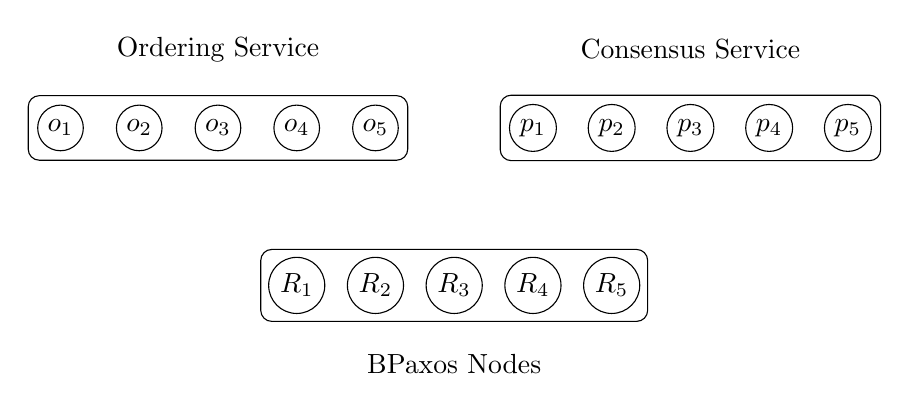
\begin{tikzpicture}
    \tikzstyle{machine}=[draw, circle, inner sep=2pt]

    % Ordering Service
    \node[machine] (o1) at (0, 2) {$o_1$};
    \node[machine] (o2) at (1, 2) {$o_2$};
    \node[machine] (o3) at (2, 2) {$o_3$};
    \node[machine] (o4) at (3, 2) {$o_4$};
    \node[machine] (o5) at (4, 2) {$o_5$};
    \node (os) at (2, 3) {Ordering Service};
    \draw[rounded corners]
      ($(o1.south west) + (-0.2, -0.2)$) rectangle
      ($(o5.north east) + (0.2, 0.2)$);

    % Consensus
    \node[machine] (p1) at (6, 2) {$p_1$};
    \node[machine] (p2) at (7, 2) {$p_2$};
    \node[machine] (p3) at (8, 2) {$p_3$};
    \node[machine] (p4) at (9, 2) {$p_4$};
    \node[machine] (p5) at (10, 2) {$p_5$};
    \node (os) at (8, 3) {Consensus Service};
    \draw[rounded corners]
      ($(p1.south west) + (-0.2, -0.2)$) rectangle
      ($(p5.north east) + (0.2, 0.2)$);

    % BPaxos Nodes
    \node[machine] (b1) at (3, 0) {$R_1$};
    \node[machine] (b2) at (4, 0) {$R_2$};
    \node[machine] (b3) at (5, 0) {$R_3$};
    \node[machine] (b4) at (6, 0) {$R_4$};
    \node[machine] (b5) at (7, 0) {$R_5$};
    \draw[rounded corners]
      ($(b1.south west) + (-0.2, -0.2)$) rectangle
      ($(b5.north east) + (0.2, 0.2)$);
    \node (bpaxos) at (5, -1) {BPaxos Nodes};
  \end{tikzpicture}

  \caption{BPaxos}\figlabel{BPaxos}
\end{figure}
}

\paragraph{Ordering Service}
The ordering service is responsible for computing the dependencies between
conflicting state machine commands. When a BPaxos node $R$ receives a state
machine command $a$ from a client, it chooses a unique instance $R.i$ for $a$.
Then, $R$ sends $(R.i, a)$ to the ordering service. When the ordering service
receives $(R.i, a)$, it replies with a tuple $(R.i, a, \deps{a})$ where
$\deps{a} = \set{I_1, \ldots, I_n}$ is a set of instances called $a$'s
dependencies. The ordering service maintains the following invariant.

\begin{boxedinvariant}\invlabel{OrderingService}
If two conflicting commands $a$ and $b$ in instances $I_a$ and $I_b$ yield
responses $(I_a, a, \deps{a})$ and $(I_b, b, \deps{b})$ from the ordering
service, then either $I_a \in \deps{b}$ or $I_b \in \deps{a}$ (or both). That
is, if two conflicting commands are sent to the ordering service, at least one
is guaranteed to be a dependency of the other.
\end{boxedinvariant}

There are a couple things to note about the ordering service:
\begin{itemize}
  \item
    The ordering service has a precondition that at most one command can be
    sent to the ordering service in any given instance. That is, if a BPaxos
    node sends command $(R.i, a)$ to the ordering service, then no other BPaxos
    node can send $(R.i, b)$ to the ordering service for some other command
    $b$.

  \item
    It's possible that a BPaxos node (or multiple BPaxos nodes) sends the tuple
    $(R.i, a)$ to the ordering service more than once. The ordering service
    does not guarantee that all of the responses to these requests are the
    same.  For example, BPaxos node $R$ may send $(R.1, a)$ to the ordering
    service and get a response $(R.1, a, \set{Q.1, R.2})$. Later, $Q$ might
    send $(R.1, a)$ to the ordering service and get a different response of
    $(R.1, a, \set{Q.2, R.1})$. The ordering service only provides the
    guarantees described by \invref{OrderingService}.
\end{itemize}

\newcommand{\out}{\text{out}}
Implementing a fault tolerant ordering service is straightforward. We employ
$2f + 1$ ordering service nodes $o_{1}, \ldots, o_{2f + 1}$. When a BPaxos node
$R$ sends a command $a$ in instance $R.i$ to the ordering service, it sends the
tuple $(R.i, a)$ to all $2f + 1$ of the ordering service nodes. Every ordering
service node $o_i$ maintains a directed acyclic graph $G_i$. Every vertex of
the graph is labelled with a BPaxos instance and contains a state machine
command. When $o_i$ receives a command $a$ for instance $R.i$ from a Fast
BPaxos node, it performs the following actions:
\begin{enumerate}
  \item
    Let $\out(R.i)$ be the set of outbound edges emanating from the vertex
    labelled $R.i$. If there is already a vertex in $G_i$ labelled $R.i$, then
    $o_i$ returns $(R.i, a, \out(R.i))$ and does nothing else.  Note that the
    ordering service's precondition that most one command can be sent in any
    given instance guarantees that command stored in vertex $R.i$ is $a$.
  \item
    If there does not exist a vertex labelled $R.i$ in $G_i$, then $o_i$
    inserts a vertex into $G_i$ with label $R.i$ and with command $a$. An edge
    is added from instance $R.i$ to instance $Q.j$ for every other instance
    $Q.j$ in the graph that contains a command $b$ that conflicts with $a$.
    $o_i$ then returns the tuple $(R.i, a, \out(R.i))$.
\end{enumerate}

An example of such a graph is given in
\figref{FastPaxosOrderingServiceCartoonBefore}. The same graph is shown
\figref{FastPaxosOrderingServiceCartoonAfter}, except that the command $e$ has
arrived in instance $Q.2$ and conflicts with commands $c$ and $d$.

{\begin{figure}[h]
  \centering

  \begin{subfigure}[b]{0.35\textwidth}
    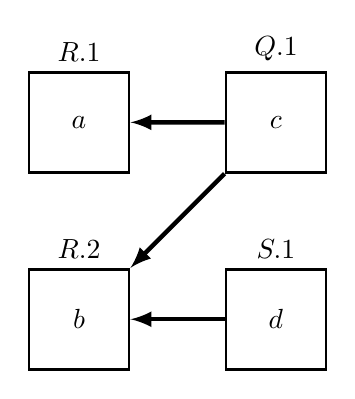
\begin{tikzpicture}[scale=2.5]
      \node[square] (a) at (0, 1) {$a$};
      \node[square] (b) at (0, 0) {$b$};
      \node[square] (c) at (1, 1) {$c$};
      \node[square] (d) at (1, 0) {$d$};
      \draw[ultra thick, -latex] (c) to (a);
      \draw[ultra thick, -latex] (c) to (b);
      \draw[ultra thick, -latex] (d) to (b);
      \foreach \label/\i in {a/$R.1$, b/$R.2$, c/$Q.1$, d/$S.1$} {%
        \node[above=0in of \label] {\i};
      }
    \end{tikzpicture}
    \caption{}\figlabel{FastPaxosOrderingServiceCartoonBefore}
  \end{subfigure}
  %
  \begin{subfigure}[b]{0.35\textwidth}
    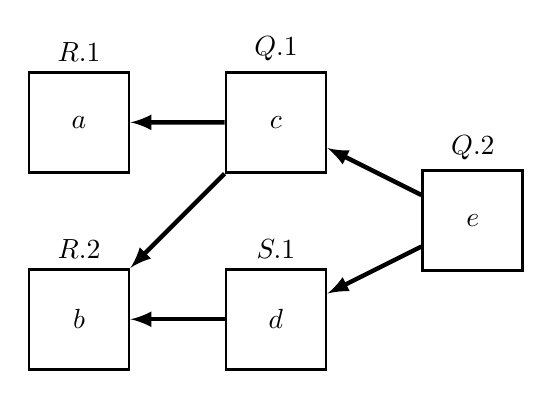
\begin{tikzpicture}[scale=2.5]
      \node[square] (a) at (0, 1) {$a$};
      \node[square] (b) at (0, 0) {$b$};
      \node[square] (c) at (1, 1) {$c$};
      \node[square] (d) at (1, 0) {$d$};
      \node[square] (e) at (2, 0.5) {$e$};
      \draw[ultra thick, -latex] (c) to (a);
      \draw[ultra thick, -latex] (c) to (b);
      \draw[ultra thick, -latex] (d) to (b);
      \draw[ultra thick, -latex] (e) to (c);
      \draw[ultra thick, -latex] (e) to (d);
      \foreach \label/\i in {a/$R.1$, b/$R.2$, c/$Q.1$, d/$S.1$, e/$Q.2$} {%
        \node[above=0in of \label] {\i};
      }
    \end{tikzpicture}
    \caption{}\figlabel{FastPaxosOrderingServiceCartoonAfter}
  \end{subfigure}

  \caption{%
    (left) A directed acyclic graph stored at a Fast BPaxos ordering service
    node. (right) The same graph after the command $e$ arrives in instance
    $Q.2$.
  }\figlabel{FastPaxosOrderingServiceCartoon}
\end{figure}

}

There are a couple of things worth noting about an ordering service node $o_i$
and the corresponding graph $G_i$.
\begin{itemize}
  \item
    $G_i$ is always acyclic.
  \item
    One a gadget $(I_a, a, \out(I_a))$ is inserted into $G_i$, the gadget is
    never modified.
  \item
    The edges in $G_i$ reflect the order in which conflicting commands were
    received by $o_i$. If there is an edge from instance $I_a$ to instance
    $I_b$, then $o_i$ must have received command $b$ in $I_b$ before receiving
    command $a$ in $I_a$.
  \item
    EPaxos and BPaxos both construct a directed cyclic graph of commands that
    are then executed in reverse topological order by strongly component. This
    graph is not the same graph as $G_i$.  $G_i$ is a completely separate graph
    that serves a completely different purpose.
\end{itemize}

When a BPaxos node receives replies $(R.i, a, \deps{a}_{i_1}), \ldots, (R.i, a,
\deps{a}_{i_{f+1}})$ from a quorum $\quorum_a$ of $f + 1$ ordering service
nodes, it takes $(R.i, a, \deps{a}_{i_1} \cup \ldots \cup \deps{a}_{i_{f+1}})$
to be the response from the ordering service. That is, it computes $\deps{a}$
by taking the union of $\deps{a}_i$ from a majority of the ordering service
nodes.

To understand why this ordering service implementation maintains
\invref{OrderingService}, consider conflicting commands $a$ and $b$ in
instances $I_a$ and $I_b$. Assume $a$'s reply $(I_a, a, \deps{a})$ was formed
from a quorum $\quorum_a$ and $b$'s reply $(I_b, b, \deps{b})$ was formed from
a quorum $\quorum_b$. Any two quorums intersect, so $\quorum_a \cap \quorum_b$
is nonempty. Let $o_i$ be an ordering service node in this intersection. $o_i$
either received $a$ or $b$ first. If it received $a$ first, then $G_i$ has a
vertex $I_a$ that contained $a$ when $o_i$ processed command $b$, so $o_i$
includes $I_a$ in $\deps{b}_i$, so $I_a$ is in $\deps{b}$. Symmetrically, if
$o_i$ received $b$ first, then it includes $I_b$ in $\deps{a}$.

\paragraph{Consensus Service}
We assume we have some set $p_1, \ldots, p_n$ of nodes that implement Plain
Jane consensus. A BPaxos node can propose to the consensus service that some
value $v$ be chosen in some instance $I$. The consensus service replies with
the value that has been chosen in instance $I$, which may or may not be $v$
depending on if there are concurrent proposers proposing to instance $i$. The
consensus service guarantees that for every instance $I$, at most one value is
ever chosen in $I$.

We can implement the consensus service with one Paxos instance for every BPaxos
instance, with consensus service nodes playing the role of Paxos acceptors and
the BPaxos nodes playing the role of Paxos proposers. Similar to MultiPaxos, we
can have each BPaxos node $R$ serve as the leader for every Paxos instance
$R.i$. Initially, $R$ runs phase 1 of Paxos for every instance $R.i$, so that
later, $R$ can get a command committed in instance $R.i$ in one round trip to
the consensus service (in the best case).

\paragraph{BPaxos Nodes}
We assume a fixed set $R_1, \ldots, R_{2f+1}$ of $2f + 1$ BPaxos nodes.
%
Clients sends state machine commands to BPaxos nodes to be executed by the
replicated state machine. When a BPaxos node $R$ receives a command $a$, it
sends the command to the ordering service in a previously unused instance $R.i$
and receives a reply $(R.i, a, \deps{a})$. $R$ then proposes the value $(a,
\deps{a})$ to the consensus service in instance $R.i$. The consensus service
then replies with some chosen value $(a', \deps{a'})$ (which is equal to $(a,
\deps{a})$ in the failure-free case). At this point, the gadget $(R.i, a',
\deps{a'})$ is considered chosen in the directed graph of state machine
commands and is eligible for execution. Node $R$ also informs the other BPaxos
nodes that the value $(a', \deps{a'})$ has been chosen.

As noted earlier, the execution of the commands in the directed graph is
identical to that of EPaxos. Committed commands are executed in reverse
topological order, one strongly connected component at a time. Within a
strongly connected component, BPaxos executes commands in an arbitrary but
deterministic order. Unlike with EPaxos, BPaxos does not annotate instances
with sequence numbers. To provide linearizability, when a BPaxos node $R$
receives command $a$ from a client, $R$ does not respond to the client until
the command $a$ has been executed by the replicated state machine. If $R$
returns to the client immediately after $a$ is chosen (as with EPaxos), then
BPaxos provides serializability instead of linearizability.

% Mention that we don't HAVE to no-op.
Note that it's possible that (1) a committed command $a$ depends on an
uncommitted instance $Q.j$, and (2) the BPaxos node $Q$ that manages the
instance $Q.j$ has crashed. If the instance $Q.j$ remains forever uncommitted,
then the command $a$ will never be executed. To avoid this liveness violation,
if any BPaxos node $R$ notices that instance $Q.j$ has been uncommitted for
some time, it can perform one of the following actions:
\begin{enumerate}
  \item
    $R$ can propose to the consensus service that the value $(\noop,
    \emptyset)$ be chosen in instance $Q.j$ where $\noop$ is a command that
    doesn't affect the state machine and doesn't conflict with any other
    command. Note that $R$ does not contact the ordering service here. $R$
    contacts the consensus service directly.

  \item
    $R$ can contact the ordering service and check if any ordering service node
    has recorded a command $b$ in instance $Q.j$. If such a command exists, $R$
    can send the tuple $(Q.j, b)$ to the ordering service, and propose the
    resulting dependencies. If no such command exists, $R$ can propose a
    $\noop$.
\end{enumerate}

\paragraph{Correctness}
BPaxos maintains \invref{GadgetsChosen} trivially because it chooses commands
using consensus. The ordering service maintains \invref{OrderingService}, which
says that the dependencies computed for conflicting commands $a$ and $b$ will
have one in the other (or both). \invref{ConflictingGadgets} says that the
dependencies of conflicting \emph{chosen} commands $a$ and $b$ will have one in
the other (or both). Thus, BPaxos nodes maintain \invref{ConflictingGadgets} by
only proposing dependencies computed by the ordering service. BPaxos nodes also
propose $\noop$'s with empty dependencies, but since $\noop$s do not conflict
with any command, \invref{ConflictingGadgets} is satisfied trivially.

Now, we discuss why \invref{GadgetsChosen} and \invref{ConflictingGadgets}
ensure BPaxos' correctness. Fortunate for us, EPaxos maintains the same two
invariants, so we can leverage EPaxos' proof of correctness. Open up
\cite{moraru2013proof} and head to section 5.6, which contains proofs of
EPaxos' correctness.
\begin{itemize}
  \item
    \textbf{Theorem 1} says that EPaxos satisfies nontriviality. Clearly, so
    does BPaxos.

  \item
    \textbf{Lemma 1} is \invref{GadgetsChosen}. As we saw, BPaxos maintains
    this invariant.

  \item
    \textbf{Theorem 2} follows from Lemma 1.

  \item
    \textbf{Theorem 3} is trivial.

  \item
    \textbf{Theorem 4} states that if two conflicting commands are both
    committed, then they will be executed in the same order by every BPaxos
    node. This follows from \invref{ConflictingGadgets}. If two commands
    conflict, then one will depend on the other or both. If both commands end
    up in the same strongly connected component, they will be executed in the
    same deterministic order. And, if the commands end up in different strongly
    connected components, then one component is guaranteed to be ordered before
    the other, so the two commands are executed in reverse topological order.
\end{itemize}

}
% {\section{An Incorrect BPaxos Variant}\seclabel{IncorrectBPaxos}
BPaxos is easy to understand, but it's inefficient. After a client sends a
state machine command to a BPaxos node, it takes two round trips (in the best
case) before the command is committed: one round trip to the ordering service
nodes and one round trip to the consensus service. In this section, we present
a simple BPaxos variant that can commit commands in one round trip (in the best
case). Unfortunately, this variant is incorrect. Still, understanding why the
variant is incorrect and how to fix it is helpful to understand the correct
BPaxos variants described below.

\paragraph{The Protocol}
First, we colocate the ordering service nodes and Paxos acceptors. This is
illustrated in \figref{ColocatedBPaxos}.
%
Second, we implement our consensus service using the Fast Paxos tweak outlined
in \algoref{FastPaxosTweak} instead of regular Paxos. As required by
\algoref{FastPaxosTweak}, we let round $0$ be a fast round and every other
round be a classic round. In Case 2 of the algorithm, a proposer determines
that a value $v$ may have been chosen in round $k$ if at least
$\QuorumMajoritySize$ acceptors in $\quorum$ voted for $v$. As before, every
BPaxos node $R$ runs phase 1 of Fast Paxos for every instance $R.i$. In the
normal case, $R$ finishes executing phase 1 and sends phase 2a ``any'' messages
to the Fast Paxos acceptors. At this point, the acceptors are free to vote for
the first proposal that they hear from anyone (not just from $R$).

{\begin{figure}[ht]
  \centering

  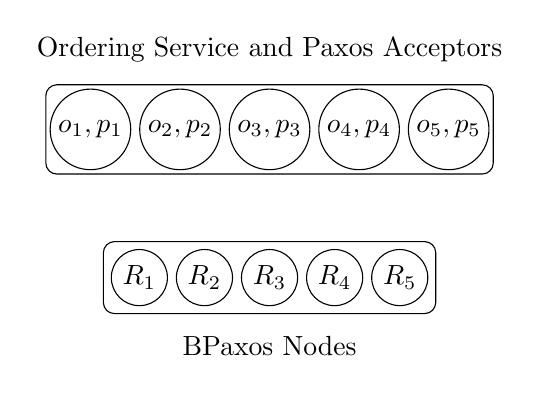
\begin{tikzpicture}
    \tikzstyle{machine}=[draw, circle, inner sep=2pt]

    % Ordering Service / Paxos Acceptors
    \node[machine] (o1) at (0, 2) {$o_1, p_1$};
    \node[machine, right=0.1cm of o1] (o2) {$o_2, p_2$};
    \node[machine, right=0.1cm of o2] (o3) {$o_3, p_3$};
    \node[machine, right=0.1cm of o3] (o4) {$o_4, p_4$};
    \node[machine, right=0.1cm of o4] (o5) {$o_5, p_5$};
    \node (os) at ($(o3.north) + (0, 0.5)$) {Ordering Service and Paxos Acceptors};
    \draw[rounded corners]
      ($(o1.south west) + (-0.2, -0.2)$) rectangle
      ($(o5.north east) + (0.2, 0.2)$);

    % BPaxos Nodes
    \node[machine, below=1cm of o3] (b3) {$R_3$};
    \node[machine, left=0.1cm of b3] (b2) {$R_2$};
    \node[machine, left=0.1cm of b2] (b1) {$R_1$};
    \node[machine, right=0.1cm of b3] (b4) {$R_4$};
    \node[machine, right=0.1cm of b4] (b5) {$R_5$};
    \draw[rounded corners]
      ($(b1.south west) + (-0.2, -0.2)$) rectangle
      ($(b5.north east) + (0.2, 0.2)$);
      \node (bpaxos) at ($(b3.south) + (0, -0.5)$) {BPaxos Nodes};
  \end{tikzpicture}

  \caption{Colocated BPaxos}\figlabel{ColocatedBPaxos}
\end{figure}
}

As before, when a BPaxos node $R$ receives a command $a$ from a client, it
sends the command to the ordering service nodes in some instance $R.i$. Upon
receiving $a$, an ordering service node $o_j$ computes its reply $(R.i, a,
\deps{a}_j)$. Unlike with BPaxos, $o_j$ does not return the reply $(R.i, a,
\deps{a}_j)$ directly to $R$. Instead, it proposes the value $(a, \deps{a}_j)$
in instance $R.i$ to $p_j$ (the colocated Fast Paxos acceptor). As we just
described, $p_j$ votes for the first proposal that it hears from anyone, so
$p_j$ votes for the value $(a, \deps{a}_j)$ in instance $R.i$ and relays its
phase 2b vote back to $R$.

If $R$ receives a superquorum (i.e.\ $f + \floor{\frac{f+1}{2}} + 1$) of phase
2b votes for the same value $(a, \deps{a}_{j_1}) = \cdots = (a,
\deps{a}_{j_m})$ in instance $R.i$, then Fast Paxos (and hence BPaxos)
considers the value chosen. Thus, in the best case, BPaxos can commit a value
in one round trip to a superquorum (just like EPaxos).

If $R$ does \emph{not} receive a superquorum of phase 2b votes for the same
value, then it is unsure whether or not a value was chosen and begins
\defword{recovery} for instance $R.i$. We'll explain recovery in one moment. At
any point in time, any other BPaxos node $Q$ may also begin recovery for
instance $R.i$. In practice, a BPaxos node will only begin recovery if it
believes $R$ has failed, but any node may attempt to recover any instance at
any time.

In this incorrect BPaxos variant, the recovery of instance $R.i$ by node $Q$ is
simply the process of $Q$ attempting to get a value chosen in $R.i$ with a
higher ballot. As with BPaxos, $Q$ can propose the value $(\noop, \emptyset)$,
or it can can contact the ordering service to see if a command $a$ has already
been proposed in instance $R.i$ and then propose $(a, \deps{a})$ where
$\deps{a}$ comes from a response from the ordering service.

\paragraph{Incorrectness}
Now, we explore why this variant of BPaxos is incorrect. Assume we are running
this BPaxos variant with $f = 2$ (i.e.\ $5$ total nodes), and imagine EPaxos
node $Q$ is attempting to recovery instance $R.i$. $Q$ begins Fast Paxos with
ballot 1 and sends phase 1a messages to some majority of consensus nodes. $Q$
receives the following phase 1b messages from a majority of acceptors:
\begin{itemize}
  \item
    $p_3$ voted for $(a, \set{I_b})$ in round $0$.
  \item
    $p_4$ voted for $(a, \set{I_b})$ in round $0$.
  \item
    $p_4$ voted for $(a, \set{I_c})$ in round $0$.
\end{itemize}
where $I_b$ is an instance with command $b$ and $I_c$ is an instance with
command $c$.
%
$Q$ then begins phase 2 of Fast Paxos. $p_3$ and $p_4$ voted for the value $(a,
\set{I_b})$ in round $0$. $p_1$ and $p_2$ maybe also voted for $(a, \set{I_b})$
in round $0$, which means that $(a, \set{I_b})$ may have been chosen in round
$0$. Thus, $Q$ executes Case 2 of \algoref{FastPaxosTweak} and proposes that
the value $(a, \set{I_b})$ be chosen.

This is incorrect! It's possible that $p_1$ and $p_2$ did \emph{not} vote for
$(a, \set{I_b})$ in round $0$. For example, they could have voted for $(a,
\set{I_c})$. In this case, $\set{I_b}$, the dependencies proposed by $Q$, is
not a response from the ordering service. Because of this, this incorrect
BPaxos variant does not maintain \invref{ConflictingGadgets}.

More concretely, we can construct the following execution of this incorrect
BPaxos variant in which two conflicting commands are both chosen and neither
depends on the other. $R$ receives command $a$ and $Q$ receives a conflicting
command $b$.  $o_1$ and $o_2$ receive $a$ and propose $(a, \emptyset)$ in
instance $R.i$ to acceptors $p_1$ and $p_2$. Similar, $o_4$ and $o_5$ receive
$b$ and propose $(b, \emptyset)$ in instance $Q.j$ to acceptors $p_4$ and
$p_5$. Then, $R$ and $Q$ crash and all other messages are dropped. Another
BPaxos node $S$ attempts to recover $R.i$. In phase 1 of Fast Paxos, it hears
from $p_1$, $p_2$, and $p_3$, and then gets the value $(a, \emptyset)$ chosen.
Then, another node $T$ recovers $Q.j$. In phase 1 of Fast Paxos, it hears from
$p_3$, $p_4$, and $p_5$ and then gets the value $(b, \emptyset)$ chosen. $S$
executes $a$ and $T$ executes $b$.

Taking a step back, we see that this BPaxos variant is incorrect because it
fails to maintain \invref{ConflictingGadgets}. It fails to maintain this
invariant because of a mismatch between the invariants that BPaxos wants to
maintain and the invariants that Fast Paxos provides. BPaxos wants to get
values of the form $(a, \deps{a})$ chosen, but only if $\deps{a}$ is a response
from the ordering service. This is required to ensure that conflicting commands
will depend on one another. However Fast Paxos wants to get \emph{any} value
chosen. Fast Paxos has no understanding of the ordering service nodes, or any
notion that some specific values should not be chosen. Fast Paxos tries to get
any proposed value chosen. In our example above, when node $S$ received 2 votes
for $(a, \emptyset)$ in round 0, Fast Paxos determined that this value may have
been chosen in round 0, so it happily proposes it. Fast Paxos doesn't
understand the additional requirement that BPaxos requires: that $(a,
\emptyset)$ cannot be chosen unless a majority of ordering service nodes
determined that $a$'s dependencies should be the empty set.

Here's another way to interpret the incorrectness of this BPaxos variant. When
a node $Q$ is recovering an instance $R.i$ and wants to propose a value $v =
(a, \deps{a})$, it has to perform the logic illustrated in
\figref{BPaxosLogic}.
%
If it's possible that a value $v$ was previously chosen, then to avoid choosing
two different values, we have no choice but to propose $v$. This is necessary
to preserve \invref{GadgetsChosen}.
%
Similarly, if $v$ is a response from the ordering service, then we're free to
propose it, but if $v$ is not a response from the ordering service, then we
can't propose it. This is necessary to preserve \invref{ConflictingGadgets}.

If a recovering node $Q$ has a value $v$ that may have been chosen \emph{and}
is maybe not a union of responses from a majority of ordering service nodes
(i.e.\ the top right corner of \figref{BPaxosLogic}), then $Q$ is stuck. It
simultaneously has to propose $v$ and cannot propose $v$. This is exactly the
situation in which our BPaxos variant is incorrect. When faced with such a
value $v$, it erroneously proposes $v$.

\begin{figure}[h]
  \centering
  \begin{tabular}{rccc}
    %
    &
    &
    \multicolumn{2}{p{3in}}{%
      Is $v$ a response from the ordering service?
    } \\
    %
    &
    &
    yes &
    maybe not \\\cline{3-4}
    %
    \multirow{2}{1.8in}{Was $v$ previously chosen?} &
    maybe &
    \multicolumn{1}{|c|}{Propose it} &
    \multicolumn{1}{|c|}{We're stuck!} \\\cline{3-4}
    %
    &
    definitely not &
    \multicolumn{1}{|c|}{Propose it, or propose noop} &
    \multicolumn{1}{|c|}{Propose noop} \\\cline{3-4}
  \end{tabular}
  \caption{The logic that any BPaxos variant should follow}%
  \figlabel{BPaxosLogic}
\end{figure}

More broadly, \figref{BPaxosLogic} illustrates the tension between preserving
\invref{GadgetsChosen} and preserving \invref{ConflictingGadgets}. Maintaining
\invref{GadgetsChosen} in isolation is easy (use Paxos), and so is maintaining
\invref{ConflictingGadgets} in isolation (use the ordering service). But,
maintaining both invariants simultaneously is tricky. There are situations,
like the top right corner of \figref{BPaxosLogic}, in which a protocol is stuck
between an \invref{GadgetsChosen} rock and an \invref{ConflictingGadgets} hard
place.

In the next couple of sections, we'll introduce a couple of BPaxos variants.
We'll see that each of these variants runs into this fundamental tension
between the two invariants, and we'll see that each variant uses a slightly
different mechanisms to deal with the tension.
}
% {\section{Unanimous Bipartisan Paxos}\seclabel{UnanimousBPaxos}
\paragraph{Overview}
Take the incorrect BPaxos variant from the previous section and increase the
Fast Paxos superquorum sizes from $f + \floor{\frac{f+1}{2}} + 1$ to $2f + 1$.
That is, choosing a value in a fast round requires a unanimous vote. We call
this variant \defword{Unanimous BPaxos}. This variant, like the incorrect
variant from the previous section, can commit a command in one round trip (in
the best case), but unlike the previous variant, this variant is correct.

\paragraph{Correctness}
Unanimous BPaxos maintains \invref{GadgetsChosen} trivially. To prove Unanimous
BPaxos maintains \invref{ConflictingGadgets}, we prove the claim $P(i)$ that
says if a Fast Paxos acceptor votes for value $(a, \deps{a})$ in round $i$,
then either
\begin{itemize}
  \item
    $i = 0$, or
  \item
    $\deps{a}$ is the union of responses from a majority of ordering service
    nodes, or
  \item
    $(a, \deps{a}) = (\noop, \emptyset)$.
\end{itemize}
We prove this by induction. $P(0)$ is trivial; the first disjunct is satisfied.
For the general case, we perform a case analysis on the proposer's logic. Call
this proposer $Q$.
\begin{itemize}
  \item (Case 1)
    $V = \set{(a, \deps{a})}$ and $k \neq 0$. $P(i)$ holds directly from
    $P(k)$.

  \item (Case 2)
    If $k \neq 0$, then $P(i)$ holds directly from $P(k)$. Otherwise, $k = 0$.
    It's only possible that value $(a, \deps{a})$ was chosen in round $0$ if
    some proposer received phase 1b messages from every acceptor such that the
    acceptors unanimously voted for $(a, \deps{a})$.

    In this case, the quorum of phase 1b messages that $Q$ received is also a
    unanimous vote for $(a, \deps{a})$.  Thus, $\deps{a}$ is the union of
    responses from a majority of ordering service nodes (the majority that $Q$
    contacted), so the second disjunct of $P(i)$ holds.

  \item (Case 3)
    In this case, a proposer always chooses to propose a $\noop$, so $P(i)$
    holds trivially.
\end{itemize}

It follows that Unanimous BPaxos maintains \invref{ConflictingGadgets} and is
therefore correct. But, let's not miss the forest through the proof. Let's take
a step back and think about why increasing the superquorum size from $f +
\floor{\frac{f+1}{2}} + 1$ to $2f+1$ turns our incorrect BPaxos variant into a
correct one. Referring to \figref{BPaxosLogic}, we see that the top right
corner is now impossible. If a Unanimous BPaxos node concludes that a value
$(a, \deps{a})$ was maybe previously chosen, then it knows for sure that
$\deps{a}$ was a union of responses from a majority of ordering service nodes.

}
% {\section{Deadlock Bipartisan Paxos}
In this section, we present \defword{Deadlock Bipartisan Paxos}. Deadlock
BPaxos can commit commands in one round trip like Unanimous BPaxos, but
Deadlock BPaxos only requires a superquorum size of $f + \floor{\frac{f}{2}} +
1$. Unfortunately, there are situations in which Deadlock Paxos can deadlock.
We will fix this pesky liveness problem in the next section.

\paragraph{Ordering Service}
Deadlock BPaxos uses the same ordering service as BPaxos and Unanimous BPaxos.

\paragraph{Consensus Service}
Deadlock BPaxos uses the same consensus service as Unanimous BPaxos, except
that Deadlock BPaxos uses a superquorums size of $f + \floor{\frac{f}{2}} + 1$,
the same as regular Fast Paxos.

\paragraph{Overview}
In the normal case, Deadlock BPaxos nodes behave exactly like Unanimous BPaxos
nodes. Upon receiving a command $a$ from a client, a Deadlock BPaxos node $R$
chooses some previously unused instance $R.i$ for the command. It then sends
$(R.i, a)$ to the ordering service nodes.
%
When an ordering service node $o_j$ receives $(R.i, a)$, it proposes it's reply
$(R.i, a, \deps{a}_j)$ to $p_j$, the colocated Paxos acceptor. $p_j$ then sends
its vote back to $R$.
%
If $R$ receives a superquorum of matching votes $(R.i, a, \deps{a})$, then the
gadget is considered chosen. If it does not receive a superquorum of matching
votes, it enters recovery.

Recovery is where Deadlock BPaxos differs from the incorrect BPaxos variant in
\secref{IncorrectBPaxos} and from Unanimous BPaxos. Deadlock BPaxos proposers
implement Case 2 and Case 3 of \algoref{FastPaxosTweak} as described in
\algoref{DeadlockBPaxos}. The bulk of the complexity comes from resolving the
tension between maintaining \invref{GadgetsChosen} and
\invref{ConflictingGadgets}, as exemplified by the upper right corner of
\figref{BPaxosLogic}.

\paragraph{Pruned Dependencies}
We'll walk through \algoref{DeadlockBPaxos} momentarily, but first we pause to
understand one of the key invariants that it maintains. Recall that in order to
preserve \invref{ConflictingGadgets}, both BPaxos and Unanimous BPaxos maintain
the invariant that a proposer can only propose a value $(a, \deps{a})$ if
either $\deps{a}$ is a response from the ordering service or if $(a, \deps{a})
= (\noop, \emptyset)$.

Deadlock BPaxos does not maintain this invariant, Instead, it maintains an
invariant that is slightly weaker but still strong enough to imply
\invref{ConflictingGadgets}. The motivation for the weaker invariant is as
follows. Imagine a Deadlock BPaxos node $R$ sends command $a$ to the ordering
service in instance $I_a$, and the ordering service responds with $(I_a, a,
\deps{a})$. Let $I_b \in \deps{a}$ be one of $a$'s dependencies. Assume that
that $R$ knows that $I_b$ has been committed with command $b$ and dependencies
$\deps{b}$. Further assume that $I_a \in \deps{b}$. That is, there is an edge
from $I_b$ to $I_a$. In this case, there is no need for $R$ to include $I_b$ in
the dependencies of $I_a$! \invref{ConflictingGadgets} asserts that if two
committed commands conflict, one has an edge to the other (or both). If $I_b$
has already committed with an edge to $I_a$, there is no need to propose an
edge from $I_a$ back to $I_b$.
%
Similarly, if $I_b$ has been committed with a $\noop$, then there is no need to
propose an edge from $I_a$ to $I_b$ at all because $a$ and $\noop$ do not
conflict.

Let $(I_a, a, \deps{a})$ be a response from the ordering service. Let
$\Pnoop{a}$ be a set of instances $I_c$ in $\deps{a}$ such that $I_c$ has been
committed as a $\noop$. Similarly, let $\Pnotnoop{a}$ be a set of instances
$I_c$ in $\deps{a}$ such that $I_c$ has been committed with $I_a$ in
$\deps{c}$. Note that in this case, $c$ is not a $\noop$. We call
$\pruned(\deps{a}) = \deps{a} - (\Pnoop{a} \cup \Pnotnoop{a})$ the
\defword{pruned dependencies} of $I_a$ (or sometimes the pruned dependencies of
$a$ if $I_a$ is clear from context).  Deadlock BPaxos maintains the following
invariant:

\begin{boxedinvariant}\invlabel{PrunedDependencies}
  In Paxos instance $I_a$, A Deadlock BPaxos node will only propose a value of
  the form $(a, \pruned(\deps{a}))$ where $\pruned(\deps{a})$ is a pruned
  response from the ordering service or a value of the form $(\noop,
  \emptyset)$.
\end{boxedinvariant}

\invref{GadgetsChosen} and \invref{PrunedDependencies} imply
\invref{ConflictingGadgets}. To see why, consider two conflicting commands $a$
and $b$ chosen in instances $I_a$ and $I_b$ with pruned dependencies
$\pruned(\deps{a})$ and $\pruned(\deps{b})$ derived from unpruned dependencies
$\deps{a}$ and $\deps{b}$ from the ordering service. We want to show that $I_a
\in \pruned(\deps{a})$ or $I_b \in \pruned(\deps{a})$, or both. Note that $a$
and $b$ conflict, so we know that neither is a $\noop$ and that their unpruned
dependencies are from the ordering service.
%
By \invref{OrderingService}, either $I_b \in \deps{a}$ or $I_a \in \deps{b}$ or
both. Without loss of generality, assume $I_b \in \deps{a}$. If $I_b$ is also
in $\pruned(\deps{a})$, then we're done. Otherwise, $I_b$ has been pruned from
$\deps{a}$. This happens only if $b$ is a $\noop$ or if $I_b$ has been chosen
with $I_a \in \deps{b}$. $b$ is not a $\noop$, so $I_a \in \deps{b}$, and we're
done.

We'll see momentarily in \algoref{DeadlockBPaxos} that it's sometimes necessary
for a BPaxos node to know the sets $\Pnoop{-}$ and $\Pnotnoop{-}$ that have
been pruned from an ordering service response. Thus, BPaxos nodes propose
values of the form $(a, \pruned(\deps{a}), \Pnoop{a}, \Pnotnoop{a})$ to the
consensus service (instead of just $(a, \pruned(\deps{a}))$) where $\Pnoop{a}$
and $\Pnotnoop{a}$ were the instances pruned from $\deps{a}$ to get
$\pruned(\deps{a})$. That is, $\pruned(\deps{a}) = \deps{a} - (\Pnoop{a} \cup
\Pnotnoop{a})$. Note that when an ordering service node $o_j$ proposes value
$(a, \deps{a})$ to its colocated Fast Paxos acceptor, it actually proposes
value $(a, \deps{a}, \emptyset, \emptyset)$.

\paragraph{Deadlock BPaxos Nodes}
\begin{algorithm}[ht]
  \caption{Deadlock BPaxos recovery for instance $R.i$ (Case 2 and Case 3)}%
  \algolabel{DeadlockBPaxos}
  \begin{algorithmic}[1]
    \If{%
      $\nexists v \in V$ such that at least $\QuorumMajoritySize$ acceptors in
      $\quorum$ voted for $v$
    }
      \State propose anything that satisfies \invref{PrunedDependencies}
    \EndIf{}

    \State
    \State $(a, \deps{a}, \emptyset, \emptyset) \gets$ the value
             voted by at least $\QuorumMajoritySize$ acceptors in $\quorum$
    \State Send $(R.i, a)$ to the quorum $\quorum$ of ordering service nodes
    \State $\deps{a}' \gets$ the union of ordering service responses

    \State
    \If{$\deps{a} = \deps{a}'$}
      \State propose $(a, \deps{a}, \emptyset, \emptyset)$
    \EndIf{}

    \State
    \State $\Pnoop{a} \gets \emptyset$
    \State $\Pnotnoop{a} \gets \emptyset$
    \For{$I_b \in \deps{a}' - \deps{a}$}
      \If{$I_b$ not committed}
        \State recover $I_b$
      \EndIf
      \If{$I_b$ committed with $\noop$}
      \State $\Pnoop{a} \gets \Pnoop{a} \cup \set{I_b}$
        \State continue
      \EndIf{}
      \If{$I_b$ committed with $R.i \in \pruned(\deps{b})$}
        \Comment{$b \to a$ unpruned}
        \State $\Pnotnoop{a} \gets \Pnotnoop{a} \cup \set{I_b}$
        \State continue
      \ElsIf{$I_b$ committed with $R.i \notin \Pnotnoop{b}$}
        \Comment{$b \not\to a$}
        \State propose anything that satisfies \invref{PrunedDependencies}
      \Else{}
        \Comment{$b \not\to a$ pruned}
        \State $I_b$ committed with $R.i \in \Pnotnoop{b}$
        \State abort recovery; $R.i$ has already been chosen
      \EndIf{}
    \EndFor{}
    \State propose $(a, \deps{a}, \Pnoop{a}, \Pnotnoop{a})$
  \end{algorithmic}
\end{algorithm}

Now, we walk through \algoref{DeadlockBPaxos} for a Deadlock BPaxos node $S$
recovering instance $R.i$. If there does not exist a value $v \in V$ with at
least $\QuorumMajoritySize$ votes from acceptors in $\quorum$, then no value
could have been chosen in round $0$, so $S$ is free to propose anything, so
long as it satisfies \invref{PrunedDependencies}.

Otherwise, there is some $(a, \deps{a}, \emptyset, \emptyset)$ that was voted
by a majority of $\quorum$. We know that $\deps{a}$ is unpruned and that
$\Pnoop{a} = \Pnotnoop{a} = \emptyset$ because this value was proposed by an
ordering service node in round $0$.
%
As we saw with the incorrect BPaxos variant in \secref{IncorrectBPaxos}, we
cannot blindly propose $(a, \deps{a})$ because it's possible that $\deps{a}$ is
not a response from the ordering service.  Thus, $S$ has to do a bit of
detective work to determine either that $\deps{a}$ is indeed a response from
the ordering service or that $(a, \deps{a}, \emptyset, \emptyset)$ was
definitely not chosen.

First, $S$ sends $(R.i, a)$ to every ordering service node in $\quorum$ and
gathers the union of their responses, $\deps{a}'$. Note that these requests can
be piggybacked on the phase 1a messages previously sent by $S$ to eliminate the
extra round trip. A majority of the acceptors in $\quorum$ voted for
$\deps{a}$, and $\deps{a}'$ is a union of these responses (and the responses
from the other acceptors in $\quorum$), so $\deps{a}'$ is either equal to
$\deps{a}$ or a superset of $\deps{a}$.

If $\deps{a} = \deps{a}'$, then $\deps{a}$ is a response from the ordering
service, so $S$ is free to propose it. Otherwise, $\deps{a}'$ is a superset of
$\deps{a}$. $S$ then enters a for loop in an attempt to prune $\deps{a}'$ until
it's either equal to $\deps{a}$ or until it determines that $\deps{a}$ could
not have been chosen in the first place.

For every, $I_b \in \deps{a}' - \deps{a}$, $S$ first gets $I_b$ committed if it
isn't already. To commit $I_b$, $S$ simply begins the recovery process for
$I_b$. If $I_b$ is a $\noop$ or if $R.i \in \pruned(\deps{b})$, then we can
prune $I_b$ and move on to the next $I_b$. Otherwise, $I_b$ is not a $\noop$
and is committed without $R.i \in \pruned(\deps{b})$. Now, $\pruned(\deps{b})$
is a (possibly) pruned response from the ordering service. Let the
corresponding unpruned dependencies be $\deps{b}$. We perform a case analysis
on whether $R.i \in \deps{b}$.
\begin{itemize}
  \item \textbf{Case $R.i \notin \deps{b}$.}
    If $R.i \notin \deps{b}$ (equivalently $R.i \notin \Pnotnoop{b}$), then
    there is some quorum of ordering service nodes that processed $I_b$ before
    $R.i$. Then, it is impossible for there to be a superquorum of nodes that
    processed $R.i$ before $I_b$. Thus, $\deps{a}$ cannot have been chosen on
    the fast path in round $0$. In this case, we are free to propose anything.

  \item \textbf{Case $R.i \in \deps{b}$.}
    If $R.i \in \deps{b}$ (equivalently $R.i \in \Pnotnoop{b}$), then it has
    been pruned from $\deps{b}$. Thus, either $R.i$ has been committed as a
    $\noop$ or $R.i$ has been committed with $I_b$ in the pruned dependencies
    of $I_a$. In either case, $R.i$ has already been committed, so we abort
    recovery for $R.i$.
\end{itemize}

Finally, if $S$ exits the for loop, then it has pruned $\deps{a}'$ into
$\deps{a}$ and can now propose it.

\paragraph{Correctness}
Deadlock BPaxos satisfies \invref{GadgetsChosen} by using Fast Paxos. It
satisfies \invref{ConflictingGadgets} by satisfying
\invref{PrunedDependencies}. It satisfies \invref{PrunedDependencies} because
every proposal issued in \algoref{DeadlockBPaxos} is a proposal for $\noop$ or
a pruned response from the ordering service.

\paragraph{Deadlock}
While Deadlock BPaxos is correct, as its name suggests, it is not very live.
There are certain situations in which BPaxos can permanently deadlock. The
reason for this is as follows. When a Deadlock BPaxos node $S$ recovers
instance $I_a$, it may have to first recover instance $I_b$. When $S$ recovers
instance $I_b$, it may have to recover $I_c$. And, when $S$ recovers $I_c$, it
may have to recover $I_a$! At this point $S$ is deadlocked.

More concretely, consider a Deadlock BPaxos deployment with $9$ nodes ($f =
4$). Imagine $4$ of these nodes have failed. The state of the remaining
ordering service nodes are shown in \figref{DeadlockBPaxosExample}. All five
ordering service nodes have processed five events $0$ through $4$ in instances
$I_0$ through $I_4$. Every command $i$ conflicts with $i - 1 \bmod 5$ and $i +
1 \bmod 5$. For example, $0$ conflicts with $4$ and $1$. Ordering service node
$o_1$ has seen the five commands in the order $0, 1, 2, 3, 4$, ordering service
node $o_2$ has seen the five commands in the order $1, 2, 3, 4, 0$, and so on.

{

\begin{figure}[ht]
  \centering

  \tikzstyle{smallsquare}=[
    draw,
    line width=1pt,
    minimum height=0.25in,
    minimum width=0.25in,
  ]

  \tikzstyle{dep}=[
    -latex,
    ultra thick,
  ]

  \begin{subfigure}[b]{0.3\textwidth}
    \centering
    \begin{tikzpicture}[xscale=1.1]
      \foreach \i [count=\x] in {0, 1, 2, 3, 4} {%
        \node[smallsquare] (\i) at (\x, 0) {$\i$};
      }
      \draw[dep] (1) to (0);
      \draw[dep] (2) to (1);
      \draw[dep] (3) to (2);
      \draw[dep, bend right] (4) to (0);
      \draw[dep] (4) to (3);
    \end{tikzpicture}
    \caption{$G_1$}\figlabel{DeadlockBPaxosExampleG1}
  \end{subfigure}
  \hspace{1in}%
  \begin{subfigure}[b]{0.3\textwidth}
    \centering
    \begin{tikzpicture}[xscale=1.1]
      \foreach \i [count=\x] in {1, 2, 3, 4, 0} {%
        \node[smallsquare] (\i) at (\x, 0) {$\i$};
      }
      \draw[dep, bend right] (0) to (1);
      \draw[dep] (0) to (4);
      \draw[dep] (2) to (1);
      \draw[dep] (3) to (2);
      \draw[dep] (4) to (3);
    \end{tikzpicture}
    \caption{$G_2$}\figlabel{DeadlockBPaxosExampleG2}
  \end{subfigure}

  \vspace{0.2in}

  \begin{subfigure}[b]{0.3\textwidth}
    \centering
    \begin{tikzpicture}[xscale=1.1]
      \foreach \i [count=\x] in {2, 3, 4, 0, 1} {%
        \node[smallsquare] (\i) at (\x, 0) {$\i$};
      }
      \draw[dep] (0) to (4);
      \draw[dep] (1) to (0);
      \draw[dep, bend right] (1) to (2);
      \draw[dep] (3) to (2);
      \draw[dep] (4) to (3);
    \end{tikzpicture}
    \caption{$G_3$}\figlabel{DeadlockBPaxosExampleG3}
  \end{subfigure}
  \hspace{1in}%
  \begin{subfigure}[b]{0.3\textwidth}
    \centering
    \begin{tikzpicture}[xscale=1.1]
      \foreach \i [count=\x] in {3, 4, 0, 1, 2} {%
        \node[smallsquare] (\i) at (\x, 0) {$\i$};
      }
      \draw[dep] (0) to (4);
      \draw[dep] (1) to (0);
      \draw[dep] (2) to (1);
      \draw[dep, bend right] (2) to (3);
      \draw[dep] (4) to (3);
    \end{tikzpicture}
    \caption{$G_4$}\figlabel{DeadlockBPaxosExampleG4}
  \end{subfigure}

  \vspace{0.2in}

  \begin{subfigure}[b]{0.3\textwidth}
    \centering
    \begin{tikzpicture}[xscale=1.1]
      \foreach \i [count=\x] in {4, 0, 1, 2, 3} {%
        \node[smallsquare] (\i) at (\x, 0) {$\i$};
      }
      \draw[dep] (0) to (4);
      \draw[dep] (1) to (0);
      \draw[dep] (2) to (1);
      \draw[dep] (3) to (2);
      \draw[dep, bend right] (3) to (4);
    \end{tikzpicture}
    \caption{$G_5$}\figlabel{DeadlockBPaxosExampleG5}
  \end{subfigure}

  \caption{A Deadlock BPaxos deadlock}%
  \figlabel{DeadlockBPaxosExample}
\end{figure}
}

Imagine BPaxos node $S$ attempts to recover $I_0$. $\QuorumMajoritySize$
acceptors have voted for $\deps{0} = \set{4}$, but $o_2$ voted for $\set{1,
4}$. Thus, $S$ attempts to recover $I_1$. $\QuorumMajoritySize$ acceptors have
voted for $\deps{1} = \set{0}$, but $o_3$ voted for $\set{0, 2}$, so $S$
attempts to recover $I_2$. This continues until $S$ attempts to recover $I_4$.
$\QuorumMajoritySize$ acceptors have voted for $\deps{4} = \set{3}$, but $o_1$
voted for $\set{0, 3}$, so $S$ attempts to recover $I_0$. This is a deadlock.

Moreover, based on the order in which the $4$ failed nodes processed the five
commands, any four of the five commands could have been chosen. For example, if
the four failed nodes saw the commands in the order $0, 1, 2, 3, 4$, then the
commands $1, 2, 3, 4$ could have been committed on the fast path in round 0.
Or, if the four failed nodes saw the commands in the order $1, 2, 3, 4, 0$,
then the commands $2, 3, 4, 0$ could have been committed on the fast path in
round 0. Because these four nodes have failed, it is impossible for us to know
the order in which they processed the five commands, so it is impossible for us
to know which subset of the commands may have been committed. This shows that
there is no simple fix to \algoref{DeadlockBPaxos} that would allow a Deadlock
BPaxos node to resolve the deadlock.

\TODO[mwhittaker]{%
  There is still one small annoying detail not fully explained in this section.
  It might be possible that in the last else case of \algoref{DeadlockBPaxos},
  a node learns that $R.i$ has already been chosen, but it doesn't know what
  dependencies it has been chosen with. I think that this is actually
  impossible, but I'm not 100\% sure. To be super duper sure that it is
  impossible, we just have to make sure that whenever a node learns that an
  instance has been chosen, it also learns the value that was chosen. This is
  not at all hard to do, but it makes the protocol a little bit more
  cumbersome.
}
}
% {\section{Majority Commit BPaxos}


\TODO[mwhittaker]{%
  Complete this section. In short, Majority Commit BPaxos fixes the deadlock
  issues that Deadlock BPaxos has.
}
\TODO[mwhittaker]{%
  Check if EPaxos is susceptible to the deadlock issues that Deadlock BPaxos
  has. The EPaxos proof of deadlock freedom seems like it might have a bug in
  it.
}

\TODO[mwhittaker]{%
  Explain that Unanimous BPaxos, Deadlock BPaxos, and Majority Commit BPaxos
  can be "fast" in the sense of Fast Paxos. Clients can initiate the protocol.
  They don't have to send to a command leader first. The one wrinkle is that a
  client will have to randomly pick a leader for the instance, say $R$, and
  send the command in some fresh instance owned by $R$. These fresh instances
  have to be default initialized in the any state, but this doesn't affect the
  correctness of anything.
}

\TODO[mwhittaker]{%
  Explain how EPaxos gets quorum sizes one smaller. Explain why EPaxos cannot
  be "fast" and why that affects the protocol in non-trivial ways.
}

\TODO[mwhittaker]{%
  Think about a Caesar variant of BPaxos. BPaxos may not satisfy the two main
  invariants. It seems like they don't run consensus on edges, only on
  commands?
}
}
{\section{Correctness}
When we say that BPaxos is ``correct'', what do we mean? In this section, we'll
answer this question.

\subsection{Generalized Consensus on Logs}
In~\cite{lamport2005generalized}, Lamport introduces \defword{generalized
consensus}, a formalism that captures our intuition of what it means for a
consensus protocol to be correct. Generalized consensus is, as the name
implies, very general. It can be used to reason about consensus on logs, on
sets, on dependency graphs, you name it. Discussing generalized consensus in
full generality, requires us to define a new algebraic structure called a
\defword{command structure set}, or CStruct for short. These details get a bit
intense, and for our purposes, we don't need to discuss generalized consensus
in full generality. So, we'll skip the details and focus on two particular
instances of generalized consensus: generalized consensus on logs and
generalized consensus on traces.

\newcommand{\Cmd}{\Sigma}
\newcommand{\prefixof}{\sqsubseteq}
First up, \defword{generalized consensus on logs}. Protocols like MultiPaxos
and Raft implement consensus on logs. All replicas agree on a totally ordered
sequence of commands (called a log) that they all execute in exactly the same
order. Formally, let $\Cmd$ be a set of commands. A \defword{log} $x \in
\Cmd^*$ is simply a string of commands. We write $x \prefixof y$ to denote that
$x$ is a prefix of $y$, and we say that $z$ is an upper bound of $x$ and $y$ if
$x \prefixof z$ and $y \prefixof z$. A log consensus protocol (e.g.,
MultiPaxos, Raft) involves a set of clients that propose commands and a set of
learners that learn the state of the log over time. We say such a protocol
implements generalized consensus on logs if it satisfies the following
properties:
\begin{itemize}
  \item \textbf{Nontriviality:}
    At every point in time, the log $x$ learned by a learner can only contain
    commands proposed by a client.

  \item \textbf{Stability:}
    If a learner learns log $x$ at one point in time and log $y$ at a later
    point in time, then $x \prefixof y$. That is, a learner's log only grows
    over time.

  \item \textbf{Consistency:}
    For any two logs $x$ and $y$ learned by two different learners, there
    exists some upper bound of $x$ and $y$. That is, at any point in time two
    logs may not necessarily be equal, but they can be extended to be equal.

  \item \textbf{Liveness:}
    If a command is proposed, it eventually appears in a learned log.
\end{itemize}

Note that consistency allows two learners to have different logs so long as the
two logs can be extended to be equal. For example, logs $ab$ and $abcd$ are not
equal, but we can extend $ab$ to be equal to $abcd$. On the other hand, logs
$ab$ and $ba$ are not equal and \emph{cannot} be extended to be equal. In
effect, consistency forces all replicas to execute exactly the same commands in
the same order, while also allowing certain replicas to lag behind.

\subsection{Generalized Consensus on Traces}
\newcommand{\conflict}{\sim}
Next up, \defword{generalized consensus on traces}. Protocols like EPaxos,
BPaxos, Caesar, Generalized Paxos, and CURP implement consensus on traces.
Instead of agreeing on a totally ordered sequence of commands, replicas agree
on a partially ordered sequence of commands in which non-conflicting commands
can be executed in any order.

We formalize traces as \defword{Mazurkiewicz
traces}~\cite{mazurkiewicz1986trace}. Again consider a set $\Cmd$ of commands.
Also consider a symmetric conflict relation $\conflict$ over $\Cmd$. We say two
commands $a, b \in \Cmd$ conflict if $a \conflict b$. Consider two strings $x,
y \in \Cmd^*$. We say $x \approx y$ if there exists $u, v \in \Sigma^*$ and
non-conflicting commands $a, b \in \Sigma$ such that $x = uabv$ and $y=ubav$.
That is, $x \approx y$ if $y$ can be derived from $x$ by swapping a single pair
of adjacent non-conflicting commands. Let $\equiv$ be the symmetric,
transitive, reflexive closure of $\approx$. We say two strings are equivalent
if $x \equiv y$. Let $[x]$ be the equivalence class of string $x$ under
$\equiv$. We call $[x]$ a Mazurkiewicz trace. The set of all Mazurkiewicz
traces is the quotient $\Cmd/\equiv$ which is equal to $\setst{[x]}{x \in
\Sigma^*}$.

More informally, a Mazurkiewicz trace is a string of commands, except that we
are allowed to repeatedly replace adjacent non-conflicting commands. For
example, letting $\Cmd = \set{a, b, c, d}$ with $a \conflict b$, $a \conflict
c$, and $a \conflict d$, we have
\[
  abcd \approx abdc \approx adbc \approx adcb
\]
so $abcd$, $abdc$, $adbc$, and $adcb$ are all equivalent. They all represent
the same Mazurkiewicz trace. That is,
\[
  [abcd] = [abdc] = [adbc] = [adcb]
\]

Note that Mazurkiewicz traces appear in a lot of areas of computer science,
though often not under the same name. For example, the theory of database
serializability uses identical definitions to describe things like transaction
histories, conflicting reads and writes, and equivalent serial orders.  Also
note that Lamport calls Mazurkiewicz traces command
histories~\cite{lamport2005generalized}.

Another important bit of theory is that Mazurkiewicz traces are isomorphic to
dependency graphs. A \defword{dependency graph} $G = (V, E, \phi)$ is an
acyclic directed graph $(V, E)$ with a function $\phi: V \to \Cmd$ that labels
each vertex with a command. The dependency graph corresponding to Mazurkiewicz
trace $[a_1 a_2 \ldots a_n]$ has $n$ vertices labelled $a_1, \ldots, a_n$. The
vertex labelled $a_i$ has an edge to every vertex labelled $a_j$ where $j < i$
and $a_i \conflict a_j$. Conversely, The Mazurkiewicz trace corresponding to a
dependency graph can be formed by topologically sorting the graph. Considering
the example from above, the trace $[abca]$ has the following dependency graph:
\begin{center}
  \tikzstyle{vert}=[draw, thick]
  \tikzstyle{dep}=[-latex, thick]
  \begin{tikzpicture}
    \node (a0) at (0, 0) {$a$};
    \node (b) at (1, 1) {$b$};
    \node (c) at (1, -1) {$c$};
    \node (a1) at (2, 0) {$a$};
    \draw[dep] (b) to (a0);
    \draw[dep] (c) to (a0);
    \draw[dep] (a1) to (b);
    \draw[dep] (a1) to (c);
  \end{tikzpicture}
\end{center}
Topologically sorting the graph, we get strings $abca$ or $acba$, which
are equivalent.

Now that we've formalized traces and dependency graphs, we return to
generalized consensus. We write $[x] \prefixof [y]$ to denote that trace $[x]$
is a prefix of trace $[y]$ (that is, there exists some $z \in \Cmd^*$ such that
$[xz] = [y]$).  We say $[z]$ is an upper bound of $[x]$ and $[y]$ if $[x]
\prefixof [z]$ and $[y] \prefixof [z]$. A trace consensus protocol (e.g.,
EPaxos, BPaxos, Generalized Paxos) involves a set of clients that propose
commands and a set of learners that learn the state of the trace over time. We
say such a protocol implements generalized consensus on traces (or command
histories) if it satisfies the following properties:
\begin{itemize}
  \item \textbf{Nontriviality:}
    At every point in time, the trace $[x]$ learned by a learner can only
    contain commands proposed by a client.

  \item \textbf{Stability:}
    If a learner learns trace $[x]$ at one point in time and trace $[y]$ at a
    later point in time, then $[x] \prefixof [y]$. That is, a learner's trace
    only grows over time.

  \item \textbf{Consistency:}
    For any two traces $[x]$ and $[y]$ learned by two different learners, there
    exists some upper bound of $[x]$ and $[y]$. That is, at any point in time
    two traces may not necessarily be equal, but they can be extended to be
    equal.

  \item \textbf{Liveness:}
    If a command is proposed, it eventually appears in a learned trace.
\end{itemize}

Note that the correctness criteria of generalized consensus on logs and the
correctness criteria of generalized consensus on traces are more or less the
same.
%
Moreover, if we write $x \prefixof y$ to denote that dependency graph $x$ is a
prefix of dependency graph $y$, and if we say $z$ is an upper bound of $x$ and
$y$ if $x \prefixof z$ and $y \prefixof z$, then we can define generalized
consensus on dependency graphs exactly as we did for traces. Generalized
consensus on traces and generalized consensus on dependency graphs are exactly
the same thing.

\subsection{EPaxos Correctness Criteria}
Generalized consensus has a lot of attractive qualities. It's formal but
intuitive. It's general. It's been around for a while. Ideally, researchers
would invent new consensus protocols that implement generalized consensus and
not bother inventing new correctness criteria for every new protocol. And in
fact, since Lamport introduced generalized consensus, this has largely been the
case. Generalized Paxos uses generalized consensus. GPaxos uses generalized
consensus. BPaxos uses generalized consensus. So does Caesar.

However, EPaxos notably does not use it. Instead, EPaxos implements a new set
of correctness criteria with definitions of nontrivialty, stability,
consistency, execution consistency, execution linearizability, and liveness.
Nontriviality, stability, and liveness are essentially the same as in
generalized consensus. Execution linearizability is just linearizability, a
nice property to add. Consistency is an implementation detail of EPaxos. The
most interesting criterion is execution consistency which is defined as ``If
two interfering commands $\gamma$ and $\delta$ are successfully committed (by
any replicas) they will be executed in the same order by every replica''.

Execution consistency replaces generalized consensus' definition of
consistency. The new definition, unfortunately, has a couple of flaws.
\begin{itemize}
  \item
    First, commands can be executed multiple times, but the definition of
    execution consistency does not disambiguate between repeated commands.
    For example, if a replica executes $\gamma$ then $\delta$ then $\gamma$
    again, did it execute $\gamma$ before $\delta$ or after?
  \item
    Second, execution consistency is defined with a sense of liveness in it.
    It says commands ``will be executed''. It's preferable to separate out
    safety properties from liveness properties.
  \item
    Third, the distinction between committing a command and executing a command
    is an implementation detail of EPaxos. Ideally, the correctness criterion
    would not rely on this implementation detail.
  \item
    Finally, it's unclear how EPaxos' correctness criteria relate to those of
    generalized consensus. Are the two equivalent? If not, how do they differ?
\end{itemize}

However, these flaws are largely minor and pedantic.  EPaxos' correctness
criteria have the major advantage of simplicity.  The new definitions are
\emph{much} simpler to digest than a full blown description of generalized
consensus. The EPaxos paper doesn't have to define traces or dependency graphs,
it doesn't have to discuss prefixing or upper bounds, and it doesn't have to
introduce generalized consensus at all. The new criteria get to the heart of
the matter: conflicting commands should be executed in the same order on all
replicas.

\subsection{Reconciling Generalized Consensus and EPaxos}
In this section, we give EPaxos' correctness criteria a face lift. We formalize
execution consistency and prove that it is equivalent to generalized consensus'
consistency.

\newcommand{\happensbefore}{<}
\newcommand{\couldhappenbefore}{<_?}
First, we formalize the notion that one replica executes one command before
another. EPaxos and BPaxos replicas sequentially execute commands. These
commands form a trace $[a_1 \ldots a_n]$. The trace may contain duplicate
commands but fortunately, every command is chosen in a unique instance. Thus,
we can essentially think of the commands as unique, where command $a$ chosen in
instance $I$ is different from command $a$ chosen in instance $J$.

Let $[x]$ be such a trace. Let $a$ and $b$ be conflicting commands. We say that
\defword{$a$ happens before $b$ in $[x]$}, denoted $a \happensbefore b$ in
$[x]$, if $a, b \in x$ and $a$ precedes $b$ in $x$ or if $a \in x$ and $b
\notin x$.  Note that if $a$ and $b$ did not conflict, the notion of $a$
preceding $b$ in $x$ would be ill-defined since $a$ could precede $b$ in $x$
but not $y$ where $[x] = [y]$. Similarly, we say that \defword{$a$ could happen
before $b$ in $[x]$}, denoted $x \couldhappenbefore b$ in $[x]$, if $a
\happensbefore b$ in $[x]$ or if $a, b \notin x$. For example, consider the
following trace, where all commands conflict:

\[
  [x] = [ab]
\]

In this trace, $a \happensbefore b$, $a \couldhappenbefore b$, $a
\happensbefore c$, $a \couldhappenbefore c$, and $c \couldhappenbefore d$. It
is not the case that $b \happensbefore a$, $b \couldhappenbefore a$, or $c
\happensbefore d$.

Now, we formalized execution consistency. For any two traces $[x]$ and $[y]$
executed by two replicas, and for any two conflicting commands $a$ and $b$, if
$a \happensbefore b$ in $[x]$ then $a \couldhappenbefore b$ in $[y]$.

\begin{theorem}\thmlabel{epaxos_genpaxos_equivalence}
  Execution consistency and generalized consensus' consistency are equivalent.
  That is, for any two traces $[x]$ and $[y]$ with unique commands and for any
  conflicting commands $a$ and $b$, the following two are equivalent:
  \begin{itemize}
    \item
      $a \happensbefore b$ in $[x]$ implies $a \couldhappenbefore b$ in $[y]$
      and
      $a \happensbefore b$ in $[y]$ implies $a \couldhappenbefore b$ in $[x]$.
    \item
      $[x]$ and $[y]$ have an upper bound.
  \end{itemize}
\end{theorem}
\begin{proof}
  First, we prove the forward direction. For strings $u, v$, let $u - v$ be the
  commands that appear in $u$ but not $v$, in the order they appear in $u$. For
  example, $abcd - bd = ac$. We show that $[x(y-x)] = [y(x-y)]$. $x(y-x)$ and
  $y(x-y)$ are permutations, so by \lemref{trace_permutation}, it suffices to
  show that $x(y-x)$ orders conflicting commands the same as $y(x-y)$. Let $a,
  b \in x$ be conflicting commands in $x(y-x)$ where $a$ precedes $b$.
  \begin{itemize}
    \item \textbf{Case $a, b \in x$.}
      \begin{itemize}
        \item \textbf{Case $a, b \in y$.}
          $a \happensbefore b$ in $[x]$, so $a \couldhappenbefore b$ in $[y]$.
          $a, b \in y$, so $a$ precedes $b$ in $y(x-y)$.

        \item \textbf{Case $a \in y, b \notin y$.}
          $a \in y$ and $b \in (x-y)$, so $a$ precedes $b$ in $y(x-y)$.

        \item \textbf{Case $b \in y, a \notin y$.}
          $a \happensbefore b$ in $[x]$, but $b \happensbefore a$ in $[y]$.
          This is a contradiction.

        \item \textbf{Case $a, b \notin y$.}
          $a, b \in x-y$, so $a$ precedes $b$ in $y(x-y)$.
      \end{itemize}


    \item \textbf{Case $a \in x, b \in (y-x)$.}
      \begin{itemize}
        \item \textbf{Case $a \in y$.}
          $a \happensbefore b$ in $[x]$, so $a \happensbefore b$ in $[y]$, so
          $a$ precedes $b$ in $y(x-y)$.

        \item \textbf{Case $a \notin y$.}
          $a$ is in $x$ but not $y$, and $b$ is in $y$ but not $x$.  Thus, $a
          \happensbefore b$ in $[x]$, but $b \happensbefore a$ in $[y]$. This
          is a contradiction.
      \end{itemize}


    \item \textbf{Case $a, b \in (y-x)$.}
      $a$ precedes $b$ in $y$, so $a$ precedes $b$ in $y(x-y)$.
  \end{itemize}

  Next, the reverse direction. First note that if $a \happensbefore b$ in trace
  $[w]$, then $a \happensbefore b$ in all suffixes of $[w]$. Similarly, if $a
  \happensbefore b$ in trace $[w]$, then $a \couldhappenbefore b$ in all
  prefixes of $[w]$.
  %
  Let $[z] = [xz_x] = [yz_y]$ be the upper bound of $[x]$ and $[y]$. Assume $a
  \happensbefore b$ in $[x]$. $a \happensbefore b$ in $[x]$, so $a
  \happensbefore b$ in $[xz_x]$. $[xz_x] = [yz_y]$, so $a \couldhappenbefore b$
  in $[y]$. The other direction is symmetric.
\end{proof}

\begin{lemma}\lemlabel{trace_permutation}
  Two traces $[x]$ and $[y]$ are equivalent (i.e., $[x] = [y]$) if $x$ and $y$
  are permutations that order all conflicting commands the same way.
\end{lemma}
\begin{proof}
  See Generalized Paxos~\cite{lamport2005generalized}.
\end{proof}
}
% {\section{Dependency Compaction}
}

\bibliographystyle{plain}
\bibliography{references}

% \begin{appendices}
% {\section{An Aside on Fast Paxos}\seclabel{FastPaxos}
Before we move on, we summarize the relevant bits of Fast
Paxos~\cite{lamport2006fast} that are critical to our remaining BPaxos
variants. In Fast Paxos, after a proposer receives phase 1b messages from a
quorum of acceptors, it performs the following logic to select a value to
propose:
\begin{itemize}
  \item
    Let $k$ be the largest vote round in the quorum of phase 1b messages.
    Let $V$ be the corresponding set of vote values for round $k$.
  \item
    (Case 1) If $V = \set{v}$, then propose $v$.
  \item
    (Case 2) If $V$ contains a value $v$ that may have been chosen in round
    $k$, propose $v$. Note that quorum sizes are selected in such a way that at
    most one such $v$ can exist.
  \item
    (Case 3) Otherwise, propose anything.
\end{itemize}

Proving the correctness of Fast Paxos involves proving the statement $P(i)$
that says that if an acceptor votes for a value $v$ in round $i$, then no
other value besides $v$ has been or will be chosen in any round $j$ less than
$i$. We prove this claim by induction. $P(0)$ is trivial because there are no
rounds less than $0$. For the general case, we perform a case analysis on $j$.
First, assume $k \neq -1$.
\begin{itemize}
  \item
    If $k < j < i$, then no value has been or will be chosen in round $j$
    because a phase 1 quorum of acceptors had not voted in any round larger
    than $k$ and promised not to vote in any round less than $i$.

  \item
    If $k = j$, then we perform a case analysis on the proposer's logic.
    \begin{itemize}
      \item
        (Case 1) If $V = \set{v}$, then a quorum of acceptors have either voted
        for $v$ in round $k$ or promised not to vote in round $k$. Thus, no
        other value besides $v$ can be chosen in round $k$.
      \item
        (Case 2) If $V$ contains a value that may have been chosen in round
        $k$, we propose it. Quorum sizes are set up such that no other value
        could have been chosen in round $k$.
      \item
        (Case 3) No value could have been chosen in round $k$.
    \end{itemize}

  \item
    If $j < k$, we again perform a case analysis on the proposer's logic.
    \begin{itemize}
      \item
        (Case 1) By $P(k)$, no value other than $v$ has been or will be chosen
        in round $j$.
      \item
        (Case 2) Let $v_1, v_2 \in V$. By $P(v_1), P(v_2)$, no value has been
        or will be chosen in round $j$.
      \item
        (Case 3) Same as Case 2.
    \end{itemize}
\end{itemize}
If $k = -1$, then we know that no value has been or will be chosen in any round
less than $i$ by the same line of reasoning as above, so we're free to propose
anything.

Note that we can make the following small tweak to Fast Paxos without
compromising its correctness. We can change Case 1 of the proposer's logic from
``If $V = \set{v}$, then propose $v$'' to ``If $V = \set{v}$ and $k \neq 0$,
then propose $v$''. That is, a proposer will only perform Case 1 if $k \neq 0$.

\section{Reducing $\noop$s}
TODO: Mention how we can avoid sending too many noops by having BPaxos nodes
send a union of votes instead of noops.

TODO: Explain that Unanimous BPaxos and Fast BPaxos can be "fast" in the sense
of fast paxos. Clients can initiate the protocol. They don't have to send to a
command leader first. The one wrinkle is that a client will have to randomly
pick a leader for the instance, say $R$, and send the command in some fresh
instance owned by $R$. These fresh instances have to be default initialized in
the any state, but this doesn't affect the correctness of anything.
}
% \end{appendices}
\end{document}
